\documentclass{article}
\usepackage{amsmath}
\usepackage{amssymb}
\usepackage{cleveref}
\usepackage{graphicx}
\usepackage{float}
\usepackage{color, soul} 
\usepackage[small,bf]{caption}
\setlength{\captionmargin}{20pt}
\setlength{\parskip}{.5em}
\newcommand{\rednote}[1]{\textcolor{red}{#1}}
% \setlength{\parindent}{0pt}
\newcommand{\flow}{\Phi}
\newenvironment{condition}[1]
	{
	\begin{center}
	   \begin{tabular}{|p{.9\textwidth}|}
		\hline \medskip
		{\bf #1:}\\
	}
	{
		\medskip \\\hline
	\end{tabular}
	\end{center}
	}

\begin{document}

\title{Backfeed Protocol - The Objective Layer
\newline
\rednote{draft version - all comments welcome}
}
\author{Matan Field, Jelle Gerbrandy\footnote{Write to me at {\tt jelle@backfeed.cc}}, Elad Shtilerman, Primavera de Filippi}
\date{}
\maketitle

\begin{abstract}
The Backfeed protocol is a full stack operating system for the decentralized ecosystem. The protocol envisions the internal governance of single decentralized autonomous organizations (DAO) as well as the economic or other interactions between multiple DAOs. The grand vision of Backfeed is an alternate economic ecosystem in which the main agents are these decentralized entities powered by smart contracts deployed to a blockchain. In this document we focus on the basic building block of this ecosystem - the way that reputation flows in a system where a group of people vote on the value of a contribution.
\end{abstract}

\section{Introduction}

This document is the first in a series of chapters describing the several layers of the Backfeed protocol. 

We give formal analysis for the {\em objective layer} of the Backfeed Protocol or the reputation flow protocol.
It consists of a minimal set of design principles that any fully specified protocol should adhere to.
The other layers in the Backfeed stack extend the basic protocol in several directions.

The Backfeed Objective Layer Protocol describes an operating system of an organization of agents via a novel reputation system. In this organization, an agent's {\em reputation} represents her influence in the system, whereas an agent's {\em tokens} represent the economic possession within the organization. The objective protocol makes the abstraction that governance of the organization can be cast into two atomic actions, {\em contributions} and {\em evaluations}. A contribution can be anything which is of value to the organization, typical examples include code snippets, design work or content. An evaluation is an act of appraisal of a contribution done by agents. The basic logic is that once any contribution has obtained enough endorsements via evaluations then the DAO automatically rewards it with, newly minted, reputation and tokens.

This document focuses solely on the reputation aspect of the protocol.
We first sketch a general formal model  of reputation flow in the system. 
We then formulate a number of precise principles that describe how reputation should flow between different agents. Once the design principles have been laid out, we continue by a general description of the possible reputation flows and discuss the rationale in choosing from this space. A complete solution, satisfying all the requirements, in the form of code or complete mathematical specification is beyond the scope of this document.

\section{Problem Formulation}

The Backfeed Objective Layer Protocol describes a system that consists of an organization  of agents that have {\em reputation} that represents their influence in the system, and {\em tokens} that represent the property of the organization.

These agents can initiate certain actions: they can {\em make a contribution} to the organization, or {\em evaluate a previous contribution} to help determine the value (in tokens) of that contribution. These actions have effects on the distribution of reputation and tokens in the system - for example, when a contribution gets accepted on the basis of the evaluations of the agents, the contributor may be assigned tokens and reputation on the basis of the value of her contribution.

In this paper, we only focus on the flow of {\em reputation}  - we will leave the discussion of the assignment of tokens out of the equation.

We will represent our system as a labeled directed graph where the vertices are labeled by the reputation distribution over the agents and the edges are labeled with events. These events are typically actions taken by users, such as making a contribution or evaluating a previous contribution. 
%This is illustrated in \cref{fig: directed graph}.

More specifically, let $N=\{1, ..., n\}$ be a set of agents. 
A {\em reputation distribution} is a function $r: N \mapsto \mathbb{R}$ that assigns a real number $r(i)$ such that $0 \leq r(i) \leq 1$ and $\Sigma_{i \in N} r(n) = 1$.

This last condition - that the reputation of the agents sums to $1$ - is important: it represents the fact that we are interested in the influence that an agent has in making decisions together with other agents. Reputation, in this case, is not an absolute measure, but a metric that only makes sense {\em relative to the other agents}

The central idea of the Backfeed Objective Protocol is that events  that give information about the behavior of the agents  will lead do an adjustment of the reputation in the system. 
Starting from an initial reputation vector $r_0$ as ``seed'', a chain of events $e_0, ..., e_n$ may change the relative reputation of the agents involved. 
\begin{equation}
r_0 \xrightarrow{e_1} r_1 \xrightarrow{e_2} r_2 ... r_{n-1} \xrightarrow{e_n} r_n
\end{equation}

Let a {\em history}, $h$, be a sequence  $h = e_0, e_1, ...  e_n$, where each $e_i$ is an event.
We are interested in defining how reputation flows in a system as the result of a sequence of event.
To do that we define a family of functions $\flow$ that map a seed distribution $r$ and a history of events $h$ to a new reputation distribution $\flow(r, h)$. 

So our general model looks like this:
\begin{equation}
(N, E, \flow)
\end{equation}
Where $N$ is a set of agents, $E$ a set of events, and $\flow$ a function that maps reputation distributions $r: N \mapsto\mathbb{R}$ and histories $h \in \bigcup_{n\in\mathbb{N}} E^n$ to reputation distributions. 

We introduce some notation conventions and abbreviations to make formulating our conditions easier.

With regard to histories, we will not be obsessively precise, and write things like $hh'$ for the concatenation of $h$ with $h'$; or $he$ and $h(k,c,v)$ for the history $h$ appended with $e$ and $(k,c,v)$, respectively. 

We define 
\begin{equation}
\flow_{h'}(r, h) \equiv \flow(r, hh')
\end{equation}
The {\em reputation gain of $i$ from $h'$ with respect to $(r, h)$} as:
\begin{center}
 $ \Delta_{h'}(r, h)(i) \equiv \flow_{h'}(r, h)(i) - \flow(r, h)(i)$
\end{center}
An {\em evaluation} is a event in which an agent $k$ evaluates a contribution $c$ as having value $v$.
So, given a set of agents $N$, a set of contributions $C$ and a set of possible values $V$, a contribution is an element $(k,c,v) \in N \times C \times V$.
To keep the analysis manageable, in this paper we almost exclusively focus on the case where $V= \{0, 1\}$ - i.e.\ that evaluators give a simple yes/no evaluation.
Moreover, we assume that each agent only votes {\em once} for each contribution - in other words, for each agent $i$ and contribution $c$, we assume that each history contains just a single evaluation event of the form $(i, c, v)$.\footnote{The condition can be reformulated allowing for changing votes as well, but for now we will keep this simple.})
 
Although in this document, we will be concerned only with `evaluation events', we can consider other events as well. 
For example, a `contribution event' where agent $i$ makes a contribution $c$ represents an important element of the Backfeed protocol that can lead to reputation or tokens flowing the the contributor. Also, an event in which a `new agent enters the system' would make our analysis more complete.
We will leave these as objects for a future version of this document.

\section{Reputation Flow}

We will now formulate - in a formally rigorous way - a number of properties that a reputation flow function $\Phi$ should satisfy.

\subsection{Reward consensus voters}
Reputation should flow to an early evaluator in the case that a later evaluator voted the same as her.
\begin{condition}{reward consensus voters}
if $(i, c, v)$ is an evaluation in $h$ and $i \neq k$ then $\Delta_{k, c, v}(r, h)(i) \geq 0$
\end{condition}

\subsection{Reward consensus in proportion to their reputation}
Previous voters should, {\em ceteris paribus}, be rewarded in proportion to their reputation. The more reputation you have, the more reputation you gain, and the less you have, the less you can gain.
\begin{condition}{reward proportionally and linearly}
If $(i, c, v)$  and $(j, c, v)$ are evaluations in $h$, then $\Delta_{k, c, v}(r, h)(i) \geq \Delta_{k,c,v}(r', h)(j)$ if and only if $\flow(r, h)(i) \geq \flow(r', h)(j)$
\end{condition}
There is an alternative formulation of this principle, in which we do not reward the voters on the basis of their current reputation $\flow(r, h)(i)$, but on the basis of their reputation at the moment they voted.
\begin{condition}{reward proportionally on the basis of stake}
Let $h = (e_0, ..., (i, c, v), ..., (j, c, v), ..., e_n)$. Then $\Delta_{k, c, v}(r, h)(i) \geq \Delta_{k,c,v}(r', h)(j)$ if and only if $\flow(r, (e_0, ..., (i,c,v)))(i) \geq \flow(r, (e_0, ..., (j, c, v))(j)$ 
\end{condition}
However, these conditions may be too strong - the  it embodies the `rich get richer' principle, where we reward the agents with a lot of reputation more for the same action then an agent that has less reputation. We can weaken the principle by only requiring that if two agents $i$ and $j$ with $i$ having more reputation than $j$, act in the same way will not result in a situation where $j$ has more reputation than $i$.
\begin{condition}{reward proportionally}
Let $h = (e_0, ..., (i, c, v), ..., (j, c, v), ..., e_n)$. Then $\flow_{k, c, v}(r, h)(i) \geq \flow_{k,c,v}(r', h)(j)$ if and only if $\flow(r, h)(i) \geq \flow(r', h)(j)$ 
\end{condition}

\subsection{Flow should be proportional to the reputation of the evaluator}
If an evaluator has more reputation than another, then the reputation flow on the basis of an evaluation by the less influential evaluator should be less than that of a more influential evaluator:

\begin{condition}{reputation flows proportional to evaluator}
if $\flow(r, h)(k) > \flow(r, h)(l)$, then $|\Delta_{k, c, v}(r,h)(i)| \geq |\Delta_{l, c, v}(r,h)(i)|$ for each $i \not\in \{k, l \}$
\end{condition}


\subsection{Contribution Independence}

The reputation flow resulting from the evaluation of a contribution $c$ should be independent of any previous evaluation of contributions other than $c$.
\begin{condition}{contribution independence}
If $h$ and $h'$ are such that 
if, for each $i$ and $v$, it holds that $(i, c, v)  \in h$ iff  $(i, c, v) \in h'$, and if $\flow(r, h) = \flow(r', h')$, then
$\flow_{k,c,v}(r, h) = \flow_{k,c,v}(r', h')$
\end{condition}


\subsection{Time Independence}

The reputation flow as the result of an evalution to or from a previous voter $i$ should not rely on when $i$ has voted. Or, generalized, the {\em order} of the previous evaluations does not matter for calculating the reputation flow that results from the current evaluation. 
\begin{condition}{time independence}
If $h$ and $h'$ are permutations of each other, and $\flow(r, h) = \flow(r', h')$, then $\flow_{h''}(r, h) = \flow_{h''}(r, h)$
\label{condition: time independence}
\end{condition}
The reason we include this property is not because we think all protocols {\em should} behave like this. However, a $\flow$-function that is time independent greatly simplifies both the logic as well as the implementation of the protocol - it simply means we have to do a lot less of `administration' to calculate the values of $\Phi(r, h)$.

\subsection{Dynamic calculations}

We say that a protocol $\flow$ is {\em dynamic} if the reputation flow only depends on the current reputation distribution.
\begin{condition}{dynamic flow}
A protocol $\flow$ is {\em dynamic} iff for each $r$ and $r'$, if $\Phi(r, h) = \Phi(r', h)$, then $\Phi_{e}(r, h) = \Phi_{e}(r', h)$
\end{condition}
The mirror image of this property is a more `static' picture, in which reputation flow towards an agent as an effect of, for example, her vote for a contribution $c$, depends on her reputation at the moment that she voted - instead of of her current reputation. 

\begin{condition}{static flow}

Define $r^{\mbox static}_{c}(r, (e_0, ... , e_n)(i)$ be equal to $\flow(r, (e_0, ..., e_m))$ if $e_m \sim (i, c, v)$ is in $h$, and set it fo $\flow(r, h)$ otherwise. 

A protocol $\flow$ is {\em static} iff for each $r$ and $r'$, if $r^{\mbox static}_{c}(r, h) = r^{\mbox static}_{c}(r', h)$, then $\Phi_{e}(r, h) = \Phi_{e}(r', h)$
\end{condition}

\subsection{Split Insensitivity}

We envisage the system to be used in environments where users cannot be identified.
Reputation flow is potentially vulnerable to a {\em Sybil attack} in which agents try to ``game the system'' by creating many agents. This is something we want to protect against. 

Split insensitivity means that, everything else remaining equal, it should not matter that the effect on the system of two voters voting as a block (that is, always subsequently and with corresponding votes), the effect on their combined reputation is the same as the effect on the reputation of a single agent that has the same reputation as the two combined.\footnote{Our users cannot split (or merge). A more `direct' model of a Sybil attack represents also how new users enter the system (and should make it clear that it is not lucrative to have lots of new agents instead of just a single one. We can add `new-user'-events to our history and take it from there.}

To express split insensitivity, we need some notation. Let $(r, h)$ be a history for $N$, and $i$ an agent in $N$. We say that $i$ has split into $i_1$ and $i_2$ in $(r', h')$  iff $(r', h')$ is a history over $N / {i} \cup \{i_1, i_2\}$, $r'$ is just like $r$, with $r(i) = r(i_1) + r(i_2)$, and $h'$ is like $h$, but with each $(i, c, v)$ replaced with $(i_1, c, v) \cdot (i_2, c, v)$. 

If this is the case, we write $(r, h) \sim_{i/\{i_1, i_2\}} (r', h')$

\begin{condition}{strong split insensitivity} 
if $(r, h) \sim_{i/\{i_1, i_2\}} (r', h')$ then $\Delta(r, h)(i) = \Delta(r', h')(i_1) + \Delta(r'_0, h')(i_2)$
\end{condition}


\begin{condition}{split resilience}
if $(r, h) \sim_{i/\{i_1, i_2\}} (r', h')$, then $\Delta(r, h)(i) \geq \Delta(r', h')(i_1) + \Delta(r'_0, h')(i_2)$
\end{condition}

%
% {\bf weak split insensititivy}: the reputation flow after an evaluation is independent of splitting:
% \begin{center}
% if $r_k = r[k/{i,j}]_i +r[k/{i,j}]_i$, then $F(h, {\bf r})_k = F(h[k/{i,j}], {\bf r}[k/{i,j}])_i + F(h[k/{i,j}], {\bf r}[k/{i,j}])_j$
% \end{center}
Split sensitivity is a strong protection against Sybil attacks: it says that the fact that the influence an attacker has on the reputation flow depends only on the amount of reputation he controls, but is independent of the number of agents he controls. Split resilience is a weaker condition which states that an agent is better off voting as a single agent then by splitting his reputation to two or more agents. 

% Another type of Sybil attack is to create a large number of new users. As new users enter with 0 reputation, we need to make sure that these new users do not gain reputation by voting only (which is cheap): 
% \begin{center}
% If $r_i =0$, then $\Delta_e(h, {\bf r})_i = 0$
% \end{center}



\subsection{Incentivize Voting}

Those who vote should earn in confront of those who do not vote.
\begin{condition}{punish inactivity}
If $h$ is a history in which $i$ has voted on $c$, but $j$ has not, then
$\Delta_{k, c, v}(r, h)(i) > \Delta_{k, c, v}(r, h)(j)$
\label{condition:punish_non_active}
\end{condition}

\subsection{Incentivize early voting}
In the case of equal votes two evaluators with the same reputation evaluating consecutively with the same value, the first should be better off - or at least not worse off -than the second. This is an incentive for evaluating early.
\begin{condition}{Incentivize early voting}
If $\flow(r, h)(k) = \flow(r, h)(l)$ then $\flow_{(k, c, v)(l,c,v)}(r, h)(k) \geq  \flow_{(k, c, v)(l, c, v)}(r, h)(l)$
\end{condition}

\subsection{Regain your stake}
It should be possible for any evaluator to regain at least the reputation put at stake upon evaluating. In other words, if we have a system where users pay a fee for voting, then it should always be possible to regain that penalty. 
\begin{condition}{regain your stake}
For each history $h$, if $\Delta_{(k, c, v)}(r, h)(k) < 0$, then there is a history $h'$ such that $\Delta_{(k,c,v)h'}(r, h)(k) \geq 0$ 
\end{condition}


\subsection{Speed of flow}

[try to express something about how quickly reputation flows in the system - i.e.\ about `how many rounds need to pass minimally to double your rep'. Concepts like ``stability'', ``viscosity'' may be useful. This would be a measure of resilience: if there is an attack, it can only be slow. Concepts like ``stability'', ``viscosity'' may be useful.]


\subsection{Reward more for controversial votes}

Some contributions are easier to evaluate than others. For example, it is easy to reach consensus about the truth of `1+1=2', and therefore, voters should get rewarded less for voting on such decisions than voters that `stick out their neck' when voting on more difficult decisions.

We define the {\em controversiality} of a contribution $c$ in a history $h$ as the Shannon index over the votes on it's values. More precisely, for a history $h$ and a seed reputation $r_0$, let ${\mbox votes}(h, c, v)$ be equal to $\Sigma \{\Phi(r_0, h)(i)| i \mbox{ voted } v \mbox{ for } c \mbox{ in } h \}$.
\begin{equation}
\mbox{controversiality}(r_0, h, c) := - \Sigma_{v\in V} \mbox{ votes }(h, c, v) \cdot \mbox{ ln }(\mbox{ votes }(h, c, v))
\end{equation}
We can then define:
\begin{condition}{reward controversial votes}
If $\flow(r, h) = \flow(r', h')$ and $\mbox{controversiality}(r, h, c) \geq \mbox{controversiality}(r', h', c)$, then, for each $i$, $|\Delta_{k, c, v}(r, h)(i)| \geq |\Delta_{k, c, v}(r', h')(i)|$
\end{condition} 

\subsection{Resilience and Game Theory}

The concept of `resilience' of a protocol function $\flow$ pertains to the possibility of `gaming' the system, and in particular of the possibility of malign agents to gain reputation no matter what. 

Some concepts from Game Theory may be useful here. For example, a `winning strategy' for an agent is an algorithm that allows her to gain reputation in the system no matter how the other agents vote. We can say that a protocol a minimally resilient if no agent has a winning strategy.

% In specific cases - specific games - an agent will have knowledge of what the other agents will probably vote.  For example, if the object of evaluation is something that has a high probability of being uncontroversial - say our agents need to decide on a stock price at a certain time - then it is expected that fast voters will get more reputation - and in that case, a `winning strategy' may just be to vote earlier than the others. This is not a problem {\em per se}.

% If, instead, a topic is controversial, and it is hard to predict who will win, it should be difficult or impossible to find a winning strategy. 

The structure we have so far lends itself very well to a classic game theoretic analysis. We have neither time nor space to develop this in much detail in this document, but the basics will look like this.


We have not talked about who decides on the order in which agents votes. We use a standard hack from game theory and introduce `nature' or `chance' as a player for that.

The {\em reputation game defined by $\flow$ and $r_0$} then, is a rooted labeled tree. On each even node, nature chooses an agent $i$. In the next node, which we call an $i$-node, $i$ either chooses to evaluate a contribution, or passes her turn (i.e.\ she chooses not to act at all). 
We can label each even node $n$ with the value of $\flow(r_0, h)$ - where $h$ is simply the history of events that brings you from the root node to $n$.

If we identify the pay-off of the users with the reputation function (i.e. if we assume that players are only motivated by their reputation and not the decisions that are made), then what we have here is a {\em infinite-horizon extensive-form game}.

Now we can define {\em a strategy for $i$ in the game given by $r_0$ and $\flow$} as a function $S$ that assigns to each $i$-node $s$ an action $S(s)$.

We can now define the resilience of $\Phi$ like this. 

\begin{condition}{weak resilience} 
there is no winning strategy for games of arbitrary length: For each $r_0$ and each history $h$ compatible with $S$, there is an $h'$ such that $hh'$ is compatible with $S$, and $\Delta(r, hh')(i) \leq 0$.
\end{condition}
\begin{condition}{somewhat less weak resilience} 
Let $H$ be the set of histories compatible with a strategy $S$ for $i$. Then $\Sigma_{h\in H} \Delta(r, h)(i) \leq 0$
\end{condition}
A full game theoretic analysis lies beyond the scope of this document. We will just note here some directions that such an analysis could take that we think are interesting. For example, we make the pay-off function more realistic, and assume that preferences of the players not only depend on their reputation, but also on the actual value that is conferred by the decision process on the given contribution. Another ingredient to add would be ``beliefs about beliefs'' - where agents base their decisions on what they think that other players will vote.


% \section{Risks}

% \subsection{Risk: dishonest voters}

% [the ebay attack: play nicely along with the consensus until you have lots of rep - then use it to abuse the system]

% \subsection{Risk: Rich get richer}

% One problem with protocols that reward consensus is that ``the right gets richer'': if there is a large enough group of people that are aligned, reputation will continue to flow towards them until they have a majority. [say something about objective/subjective ]
% \section{The discursive dilemma}

% A result from the literature: if you vote for proposals that are logically related ('A', `B', `A or not B'), then majority voting (or any other kind of aggregation function) will give you logically inconsistent results - even if each single voter has voted consistently.
\section{Defining flow functions}

We have defined a number of formal conditions on how reputation could flow. Our task is now to explore the space of functions that satisfy these criteria.

\subsection{An example of a flow function}


We are looking for a definition of $\Phi_{k,c,v}(r, h)$.

Given contribution independence and time indepence, we know that  $\Phi_{k,c,v}(r, h)$ depends on not more information than four sets: the set $K$ consisting of the voter $\{k\}$ only, the set $O$ of agents that have not voted for $c$ yet, the set $V$ of agents that have voted $v$, and the set $-V$ of agentst that voted on $c$ with a value different from $v$.

Now to keep the definitions simple, write $r'$ for $\flow(r, h)$, and write $r'(S)$ for $\Sigma_{j\in S}\flow(r, h)(j)$

Consider now the following definition, where we have reputation flow from non-voters to previous voters:

{\bf definition: flow function}
\begin{enumerate}
\item $\Delta_{k,c,v}(r,h)(i) = 0$ if $i=k$ (current voter gains nothing)
\item $\Delta_{k,c,v}(r,h)(i) = 0$ if $i \in -V$ (different voters gain nothing)
\item $\Delta_{k,c,v}(r,h)(i) = \gamma \cdot r'(O) \cdot r'(i) / r'(V)$ 
if $i \in V$ (equal voters get some reputation from non-voters)
\item $\Delta_{k,c,v}(r,h)(i) = (1-\gamma) \cdot
r'(O)
\cdot r'(i) / 
r'(O) $ if $i \in O$ (non-voters loose some reputation)
\end{enumerate}
{\bf hypothesis:} The function $\Delta_{k, c, v}$ defined here satisfies the properties `split insensitivity', `reward consensus voters', `reward proportionally', `contribution independence',  `time independence',  `punish inactivity', `incentivize early voting'.
\begin{enumerate}
\item 

\end{enumerate}


\section{Conclusions}
[where we say what we have done, and, more importantly, what we want to do]

\end{document}
\section{Appendix}

[where we do  maths, proofs, difficult stuff]
\subsection{Split insensitivity}
In order to make the protocol split insensitive it is necessary to view any reputation $r$, regardless of who owns it, as an infinite number of infinitesimal reputation elements $dr$ so that:
\begin{equation}
r = \int_{0}^{r}\mbox{dr}.
\end{equation}

Viewed as such the process of evaluation can be seen as sequentially transferring the reputation elements of a certain agent from the ``non-voting'' compartment to the ``v - vote'' compartment. The important property which can guarantee the split insensitivity is that this happens sequentially, i.e. each reputation element transfer may trigger reputation updates to other reputation elements within different compartments. Thus evaluation occurs equally whether it is performed by a sequence of agents all voting on the same value or whether by one agent which holds the combined reputation and votes in one go.

We can therefore design what the effect of an evaluation by a reputation element $\mbox{dx}$ has on a reputation element $\mbox{dy}$ which has previously voted or not. From here on we restrict the discussion to a family of protocols in which new reputation is being generated with every evaluation and this new reputation is being awarded to previously equally voting reputation. The fact this reputation is new and is awarded to evaluators only satisfies requirement \ref{condition:punish_non_active}.

\begin{figure}[h]
	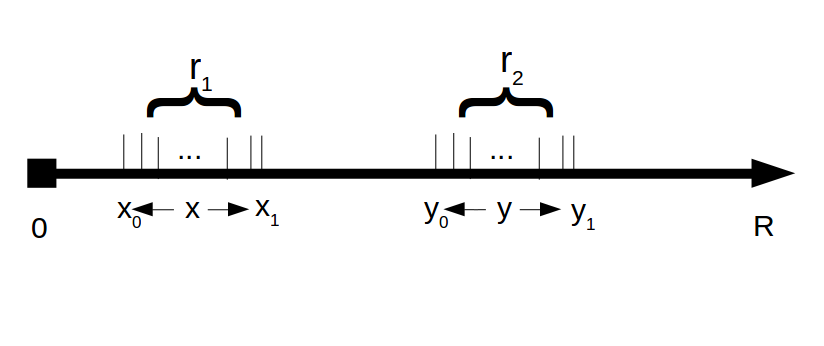
\includegraphics[width=\textwidth]{figures/reputation_arrangement.png}
	\caption{The axis of reputation in the system. The more to the right, the later the evaluation of a contribution. The figure shows the reputation of two users $r_1$ and $r_2$ as partitioned to infinitesimal fractions. $x$ runs from $x_0$ to $x_1$ so that $x_1-x_0 =r_1$ and similarly for $y$ and $r_2$. The update of $r_1$ following an evaluation by the second evaluator is the aggregated effect of all the small fractions.}
	\label{fig:rep axis}
\end{figure}

In order to continue the derivation we now postulate that when a reputation element $dy$ votes equally to a reputation element $\mbox{dx}$ which has already voted, $\mbox{dx}$ is rewarded as follows:
\begin{equation}
\mbox{dx} \rightarrow \mbox{dx}\cdot\left(1+g\cdot G(x,y,\{R_x\}\mbox{dy})\right)
\end{equation}
where $g\ll1$ is a small parameter which scales the reputation gain of a previous evaluator, $x, y$ are the ``locations'' of the reputation elements within the total reputation of their corresponding agents as shown in \cref{fig:rep axis}. $G(x,y,\{R_x\})$ reflects the dependence on the locations $x$ and $y$ and on the votes accumulated reputation distribution $\{R_x\}$. To compute the aggregate effect on the entire $r_1$ of the previous evaluator we must first calculate the entire effect of the whole $r_2$ on a single $dx$ element (of $r_1$):
\begin{subequations}
\begin{align}
\mbox{dx} \rightarrow& \mbox{dx} \cdot\prod_{y=0}^{r_2}\left(1+g\cdot G(x,y,\{R_x\})\right) \\
=& \mbox{dx}\cdot\exp\left[ \int_{0}^{r_2}\mbox{dy}\ln\left(\left(1+g\cdot G(x,y,\{R_x\})\right)\right)\right] \\
\approx& \mbox{dx}\cdot\exp\left[ g\int_{0}^{r_2}\mbox{dy}\cdot G(x,y,\{R_x\})\right]\label{eq:small g approx previous voter}\\
\approx& \mbox{dx}\cdot\exp\left[ g\int_{0}^{r_2}\mbox{dy}\cdot G(y,\{R_x\})\right]\label{eq: time indep assumption prev voter}
\end{align}
\end{subequations}
where in \cref{eq:small g approx previous voter} we assume $g\ll1$ and approximate the $\ln (...)$ to linear order and in \cref{eq: time indep assumption prev voter} we assume condition \ref{condition: time independence}. Now we can sum up this effect to get the aggregate \footnote{Note that here we are making an assumption that $\{R_x\}$ the cumulative reputation distribution does not change due to increases in reputation due to $\mbox{dx}$ being larger}:
\begin{align}
r_1 &\rightarrow \int_{0}^{r_1}\mbox{dx}\exp\left[ \int_{0}^{r_2}\mbox{dy}g\cdot G(y,\{R_x\})\right] \nonumber\\
&= r_1\cdot\exp\left[ \int_{0}^{r_2}\mbox{dy}g\cdot G(y,\{R_x\})\right] 
\label{eq:prev rep update}
\end{align}

Now given the form of the function $G(y,\{R_x\})$ we can easily calculate the reputation update for a previous evaluator with reputation $r_1$. The small $g$ approximation can be further stretched to obtain the final formula for the reputation update following an evaluation by a later evaluator:

\begin{equation}
r_1\rightarrow r_1\cdot\left[1 + g\cdot \int_{0}^{r_2}G(y,\{R_x\})\mbox{dy}\right].
\label{eq:first order in g prev}
\end{equation}
It should be noted that the dimensions of $G(y)$ are the inverse of reputation. 

We proceed to calculate the reputation update for the current evaluator. We view this process as occurring sequentially, i.e. $r_2$ is partitioned to many elements, each element gains reputation when subsequent elements execute their vote \footnote{We omit from this derivation an evaluation reputation fee or stake which needs to be payed by the current evaluator.}. Each element of $r_2$ is therefore updated as follows:
\begin{equation}
\mbox{dx}
\rightarrow
\mbox{dx}\cdot\left(1+g\cdot G(x,y,\{R_x\})\mbox{dy}\right)
\end{equation}
where now, $\mbox{dx}$ refers to an element which has voted and $\mbox{dy}$ refers to the current voting element. Note that $G(x,y,\{R_x\}) = G(y,\{R_x\})$ when $y>x$, i.e. when the element in $y$ votes after the element in $x$. When $y\le x$ $G(x,y) = 0$ i.e. only the later elements trigger reputation gain to previous elements. To compute the aggregated effect of the evaluation of $r_2$ on $r_2$ itself we write:
\begin{eqnarray}
r_2\rightarrow \int_{0}^{r_2}\mbox{dx}\cdot\exp\left(\int_{x}^{r_2}g\cdot G(y,\{R_x\})\mbox{dy}\right)
\end{eqnarray}
The second integrand reflects the fact that any element in location $x$ gains reputation following a trigger by an element in $y$ if $y>x$. Again we can continue the approximation for first order in $g$:
\begin{equation}
r_2\rightarrow \int_{0}^{r_2}\mbox{dx}\cdot\left(1+\int_{x}^{r_2}g\cdot G(y,\{R_x\})\mbox{dy}\right)
\end{equation}
Again retaining linear order in $g$ we obtain:
\begin{equation}
r_2\rightarrow r_2 +g\cdot\int_{0}^{r_2} \left(\int_{x}^{r_2}G(y,\{R_x\})\mbox{dy}\right)\mbox{dx}
\label{eq:final current eval update}
\end{equation}

\subsubsection{Worked out example}
Having specified a framework for split insensitivity we would like to test it on a simple case. Specifically, we choose a simple and reasonable form for the function $G(y,\{R_x\})$ and solve  \cref{eq:first order in g prev, eq:final current eval update} explicitly. Once these expressions are obtained, we would like to show that, to first order in $g$, the state following an evaluation by an agent with reputation $r_1+r_2$ is equivalent to the state where two agents with $r_1$ and $r_2$ vote consecutively. 	

\textbf{Need to fill in this part ...}

In that case the total reputation update for user 1 would be: 
\begin{equation}
r_1 \rightarrow r_1(1+g\log(1+\frac{r_2}{V_0}))
\end{equation}
The reputation gain for the current evaluator, user 2, needs to take into account, the fact that initially its reputation is in the non-voter compartment and during each part of the evaluation an element reputation element $dy$ is being transfered. As he accumulates reputation in the voted compartment, later reputation elements trigger reputation generation for the previous element. This results in:

\begin{equation}
r_2 \rightarrow r_2 + g(r_2 -V_0\log(1+\frac{r_2}{V_0}))
\end{equation}

It should be noted that regarding the total amount of reputation voted equally, $V_0$, then maps as follows:

\begin{equation}
V_0 \rightarrow V_0 + r_2(1+g)
\end{equation}

as the $\log$ terms cancel out. We wish to see whether this scheme is indeed split-insensitive to first order in $g$ as expected via the construction. So we assume there is an attacker which holds two users and can either vote equally with the totality of of his reputation or vote using two different users consecutively. We need to check three things:
\begin{enumerate}
	\item That the non-voters or voters voting differently are agnostic to which scenario occured. \label{non-equal_voters_condition}
	\item That previous equally voting users are also agnostic.
	\item That the total reputation gain of the attacker is equal in both scenarios.
\end{enumerate}
\Cref{non-equal_voters_condition} is trivial.




\section{References}


\begin{enumerate}
\item https://www.oasis-open.org/committees/download.php/28303/JIB2007-DSS-Survey.pdf
\end{enumerate}

\end{document}